\documentclass[11pt,fleqn]{article}
\usepackage[margin=1in]{geometry}
\usepackage{tikz}
\usepackage{mathtools}
\usepackage{longtable}
\usepackage{enumitem}
\usepackage{hyperref}
%\usepackage[dvips]{graphics}
%\usepackage[table]{xcolor}
%\usepackage{amssymb}
\usepackage{float}
%\usepackage{subfig}
\usepackage{booktabs}
\usepackage{subcaption}

\usepackage[normalem]{ulem}

\usepackage{multicol}
\usepackage{txfonts}
\usepackage{amsfonts}
%\usepackage{natbib}
\usepackage{apacite}
\usepackage{gb4e}
\usepackage[all]{xy}
\usepackage{rotating}
\usepackage{tipa}
\usepackage{multirow}
\usepackage{authblk}
\usepackage{url}
\usepackage{pdflscape}
\usepackage{rotating}
\usepackage{adjustbox}
\usepackage{array}

\definecolor{Pink}{RGB}{255,50,170}
\newcommand{\jd}[1]{\textcolor{Pink}{[jd: #1]}}  

\newcommand{\jt}[1]{\textbf{\color{blue}JT: #1}}

\newcommand{\tableref}[1]{Tab.~\ref{#1}}
\newcommand{\figref}[1]{Fig.~\ref{#1}}

\def\bad{{\leavevmode\llap{*}}}
\def\marginal{{\leavevmode\llap{?}}}
\def\verymarginal{{\leavevmode\llap{??}}}
\def\swmarginal{{\leavevmode\llap{4}}}
\def\infelic{{\leavevmode\llap{\#}}}

\definecolor{airforceblue}{rgb}{0.36, 0.54, 0.66}
%\definecolor{gray}{rgb}{0.36, 0.54, 0.66}

\newcommand{\dashrule}[1][black]{%
  \color{#1}\rule[\dimexpr.5ex-.2pt]{4pt}{.4pt}\xleaders\hbox{\rule{4pt}{0pt}\rule[\dimexpr.5ex-.2pt]{4pt}{.4pt}}\hfill\kern0pt%
}

\setlength{\parindent}{.3in}
\setlength{\parskip}{0ex}

\newcommand{\yi}{\'{\symbol{16}}}
\newcommand{\nasi}{\~{\symbol{16}}}
\newcommand{\hina}{h\nasi na}
\newcommand{\ina}{\nasi na}

\newcommand{\foc}{$_{\mbox{\small F}}$}

\hyphenation{par-ti-ci-pa-tion}

%\setlength{\bibhang}{0.5in}
%\setlength{\bibsep}{0mm}
%\bibpunct[:]{(}{)}{,}{a}{}{,}

\newcommand{\6}{\mbox{$[\hspace*{-.6mm}[$}} 
\newcommand{\9}{\mbox{$]\hspace*{-.6mm}]$}}
\newcommand{\sem}[2]{\6#1\9$^{#2}$}
\renewcommand{\ni}{\~{\i}}

\newcommand{\citepos}[1]{\citeauthor{#1}'s \citeyear{#1}}
\newcommand{\citeposs}[1]{\citeauthor{#1}'s}
\newcommand{\citetpos}[1]{\citeauthor{#1}'s \citeyear{#1}}

\newcolumntype{R}[2]{%
    >{\adjustbox{angle=#1,lap=\width-(#2)}\bgroup}%
    l%
    <{\egroup}%
}
\newcommand*\rot{\multicolumn{1}{R{90}{0em}}}% no optional argument here, please!

\title{Prior beliefs modulate projection -- Supplementary Materials}

%\thanks{For helpful comments on the research presented here, we thank the audience at the 2018 Annual Meeting of XPRAG.de and at the University of T\"ubingen. We gratefully acknowledge financial support for this research from {\em National Science Foundation} grant BCS-1452674 (JT) and the Targeted Investment for Excellence Initiative at The Ohio State University (JT). IGOR Tuebingen}}

%\author{Author(s)}

\author[$\bullet$]{Judith Degen}
\author[$\circ$]{Judith Tonhauser}

\affil[$\bullet$]{Stanford University}
\affil[$\circ$]{University of Stuttgart}

\renewcommand\Authands{ and }

\begin{document}

%\tableofcontents
%\newpage

\maketitle

\appendix

\setcounter{table}{0}
\renewcommand{\thetable}{A\arabic{table}}

\setcounter{figure}{0}
\renewcommand{\thefigure}{A\arabic{figure}}

\section{Experiment 1: Target and control stimuli}\label{a-stim}

This list shows the 20 clauses of the target stimuli alongside their lower and higher probability facts, respectively:

\begin{enumerate}[leftmargin=4ex,itemsep=-2pt]
\item Mary is pregnant. Facts: Mary is a middle school student / Mary is taking a prenatal yoga class
\item Josie went on vacation to France. Facts:  Josie doesn't have a passport / Josie loves France 
\item Emma studied on Saturday morning. Facts: Emma is in first grade / Emma is in law school 
\item Olivia sleeps until noon. Facts: Olivia has two small children / Olivia works the third shift
\item Sophia got a tattoo. Facts: Sophia is a high end fashion model / Sophia is a hipster
\item Mia drank 2 cocktails last night. Facts: Mia is a nun / Mia is a college student
\item Isabella ate a steak on Sunday. Facts: Isabella is a vegetarian / Isabella is from Argentina
\item Emily bought a car yesterday. Facts: Emily never has any money / Emily has been saving for a year
\item Grace visited her sister. Facts: Grace hates her sister / Grace loves her sister
\item Zoe calculated the tip. Facts: Zoe is 5 years old / Zoe is a math major
\item Danny ate the last cupcake. Facts: Danny is a diabetic / Danny loves cake
\item Frank got a cat. Facts: Frank is allergic to cats / Frank has always wanted a pet
\item Jackson ran 10 miles. Facts: Jackson is obese / Jackson is training for a marathon
\item Jayden rented a car. Facts: Jayden doesn't have a driver's license / Jayden's car is in the shop
\item Tony had a drink last night. Facts: Tony has been sober for 20 years / Tony really likes to party with his friends
\item Josh learned to ride a bike yesterday. Facts: Josh is a 75-year old man / Josh is a 5-year old boy
\item Owen shoveled snow last winter. Facts: Owen lives in New Orleans / Owen lives in Chicago
\item Julian dances salsa. Facts: Julian is German / Julian is Cuban
\item Jon walks to work. Facts: Jon lives 10 miles away from work / Jon lives 2 blocks away from work
\item Charley speaks Spanish. Facts: Charley lives in Korea / Charley lives in Mexico
\end{enumerate}

In the target stimuli of the projection block of Exp.~1, eventive predicates, like {\em discover} and {\em hear}, were realized in the past tense and stative predicates, like {\em know} and {\em be annoyed}, were realized in the present tense. The direct object of {\em inform} was realized by the proper name {\em Sam}. Each clause-embedding predicate was paired with a unique subject proper name. The speaker of the target stimuli was realized by a randomly sampled unique proper name. 

The following list shows the six clauses that were used in the control and filler stimuli of Exp.~1, with their facts. In the prior block, these six clauses were embedded under {\em How likely is it that\ldots?}. The projection block featured polar questions variants of the clauses.

\begin{enumerate}[leftmargin=3ex,itemsep=-2pt]
\ex Zack is coming to the meeting tomorrow. Fact: Zack is a member of the golf club. 

\ex Mary's aunt is sick. Fact: Mary visited her aunt on Sunday. 

\ex Todd played football in high school. Fact: Todd goes to the gym 3 times a week. 

\ex Vanessa is good at math. Fact: Vanessa won a prize at school. 

\ex Madison had a baby. Fact: Trish sent Madison a card. 

\ex Hendrick's car was expensive. Fact: Hendrick just bought a car. 
\end{enumerate}

\section{Data exclusion}\label{a-exclusion}

Table \ref{f-exclusion} presents how many participants' data were excluded from the analyses based on the exclusion criteria. The first column records the experiment, the second (`recruited') how many participants were recruited, and the final column (`remaining') how many participants' data entered the analysis. The `Exclusion criteria' columns show how many participants' data were excluded based on the two exclusion criteria: 

\begin{itemize}[topsep = -1ex,itemsep=-2pt]

%\item `multiple': Due to an experimental glitch, some participants participated in Exps.~1b, 2b or 3b more than once. Of these participants, we only analyzed the data from the first time they participated.

\item `language': Participants' data were excluded if they did not self-identify as native speakers of American English.

\item `controls': In Exps.~1 and 2b, participants' data were excluded if their response mean on the 6 control items was more than 2 sd above the group mean. In Exp.~2a, participants' data were excluded  if their response to (\ref{control2}a) was more than 2 sd below the group mean or if their response to (\ref{control2}b) was more than 2 sd above the group mean.

%\item `variance': Participants' data were excluded if they always selected roughly the same point on the response scale, that is, if the variance of their response distribution was more than 2 sd below the group mean variance. \jt{did we do variance or not? if not, why not?}

\end{itemize}

% exp 1 (prior, projection)
%Prior to analysis, the data from 3 participants who did not self-identify as native speakers of American English were excluded. To assess whether the remaining 297 participants attended to the task, we inspected their responses to the control stimuli. We excluded the data from 11 participants whose response means were more than 2 standard deviations above the group mean. The data from 286 participants (ages 18-82; median: 35.5; 116 female, 186 male, 1 other, 1 undeclared) were analyzed.

% exp 2a (prior):
%Prior to analysis, the data from 8 participants who did not self-identify as native speakers of American English were excluded. To assess whether the remaining 87 participants attended to the task, we inspected their responses to the 2 control stimuli. The response means of 12 participants were more than 2 standard deviations below the group mean of the control in (\ref{control}a) or more than 2 standard deviations above the group mean of the control in (\ref{control}b). We excluded the data from these participants, leaving data from 75 participants (ages 21-75; median: 35; 34 female, 41 male).

% exp 2b (projection):
%Prior to analysis, the data from 23 participants who did not self-identify as native speakers of American English were excluded. To assess whether the remaining 277 participants attended to the task, we inspected their responses to the 6 control stimuli. There were 11 participants whose response means were more than 2 standard deviations above the group mean. We excluded the data from these participants, too, leaving data from 266 participants (ages 21-72; median: 36; 129 female, 136 male, 1 undeclared).

\begin{table}[h!]
\centering
\begin{tabular}{l r | r r | r}
&  & \multicolumn{2}{c|}{Exclusion criteria} &  \\ 
&  recruited  & language & controls & remaining \\ 
\hline
Exp.~1 & 300 & 3 & 11 & 286 \\
Exp.~2a & 95 & 8 & 12 & 75 \\
Exp.~2b & 300 & 23 & 11 & 266 \\
\end{tabular}
\caption{Data exclusion in Exps.~1 and 2}\label{f-exclusion}
\end{table} 

%\section{Model details for Experiments 1 and 2}\label{modeldetails}
%
%\jt{do we need this for this journal? if not, cool, let's delete. if yes, needs to be adjusted.}
%
%This supplement provides details on the data analysis conducted for Exps.~1, 2, and 3. We first motivate the use of Beta regression rather than linear regression in Exps.~1a, 2a, and 3a (section \ref{a-motivation}) and then provide a brief primer on how to interpret Bayesian mixed effects Beta regression models (section \ref{a-primer}). We then report the model outputs for Exps.~1, 2, and 3 (section \ref{a-mo}).
%
%\subsection{Motivation for using Bayesian mixed effects Beta regression}\label{a-motivation}
%
%There are three separate pieces to motivate: the use of \emph{mixed effects}, the use of a \emph{Bayesian} rather than \emph{frequentist} models, and the use of \emph{Beta regression} rather than \emph{linear regression}. 
%
%\textbf{Using mixed effects} refers to the practice of modeling the outcome variable, here slider ratings or proportions of `yes' ratings, as a function of not just fixed effects of interest (i.e., predicate) but also as the result of possible random variability that is not of theoretical interest (e.g., random by-participant or by-item variability). This is standard practice in psycholinguistic studies and allows the researcher to trust that any observed effects of theoretical interest are true average effects rather than the result of idiosyncratic behavior (e.g., of participants or items). This is also the motivation for using mixed effects in Exps.~1b, 2b, and 3b.
%
%\textbf{Using Bayesian models} rather than frequentist models is increasingly becoming the norm in psycholinguistic studies as computational power has increased and running Bayesian models has become more accessible with the introduction of R packages such as \verb|brms| \cite{buerkner2017}. The presence of an effect in frequentist models is evaluated by checking whether the {\em p-}value is smaller than $.05$, where the {\em p-}value is defined as the probability of obtaining data that is as skewed or more skewed than the observed data if the null-hypothesis was true, i.e., if the hypothesized effect was absent. Parameter estimates in frequentist models are obtained via maximum-likelihood techniques, i.e., by estimating the parameter values that maximize the probability of observing the data. Bayesian models, by contrast, return a full posterior distribution over parameter values that take into account not just the probability of the data under the parameter values, but also the prior probability of parameter values. In order to evaluate the evidence for an effect of a predictor of interest, one can report 95\% credible intervals and the posterior probability $P(\beta < 0)$ or $P(\beta > 0)$ that the predictor coefficient $\beta$ is either lower or greater than zero, depending on the direction of the expected effect. A 95\% credible interval (CI) demarcates the range of values that comprise 95\% of probability mass of the posterior beliefs such that no value inside the CI has a lower probability than any point outside it \cite{Jaynes1976, Morey2016}. There is substantial evidence for an effect if zero is (by a reasonably clear margin) not included in the 95\% CI and $P(\beta > 0)$ or $P(\beta < 0)$ is close to zero or one. Posterior probabilities indicate the probability that the parameter has a certain value, given the data and model -- these probabilities are thus \emph{not} frequentist {\em p-}values. In order to present statistics as close to widely used frequentist practices, and following \citeNP{Nicenboim2016}, we defined an inferential criterion that seems familiar (95\%), but the strength of evidence should not be taken as having clear cut-off points (such as in a null-hypothesis significance testing framework).
%
%\textbf{Using Beta regression} rather than linear regression was motivated by the violation of two of the  assumptions of linear regression: first, that residuals be normally distributed (where ``residuals'' refers to the residual error for each data point after fitting the model), and second, that the error term exhibit homoscedasticity (that it be roughly the same across different conditions). Slider ratings data has the property of being bounded by its endpoints (which we code as 0 and 1, respectively). This often leads to ``bunching'' behavior at the endpoints (see  \figref{fig:bunch} for the distribution of raw ratings in Exps.~1a, 2a, and 3a). 
%
%
%\begin{figure}[h!]
%\begin{subfigure}{.33\textwidth}
%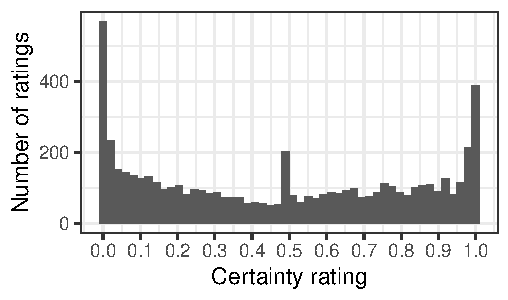
\includegraphics[width=\textwidth]{../../results/9-prior-projection/graphs/bunching-projection}
%\caption{Exp.~1 certainty ratings.}
%\label{fig:exp1araw}
%\end{subfigure}
%\begin{subfigure}{.33\textwidth}
%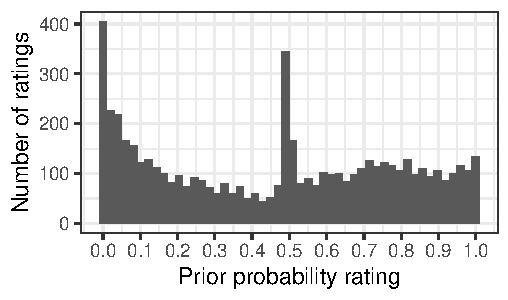
\includegraphics[width=\textwidth]{../../results/9-prior-projection/graphs/bunching-prior}
%\caption{Exp.~1 prior ratings.}
%\label{fig:exp2araw}
%\end{subfigure}
%\begin{subfigure}{.33\textwidth}
%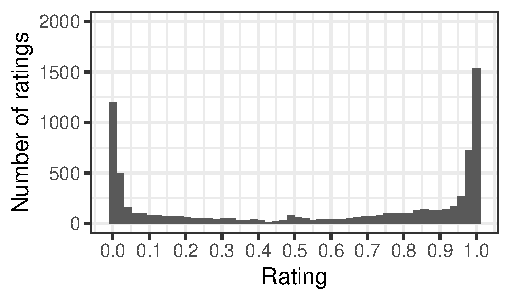
\includegraphics[width=\textwidth]{../../results/2-veridicality2/graphs/bunching}
%\caption{Exp.~2 prior ratings.}
%\label{fig:exp3araw}
%\end{subfigure}
%\caption{Histograms of raw slider ratings in Exps.~1 and 2.}
%\label{fig:bunch}
%\end{figure}
%
%This ``bunching'' behavior, in turn, can lead to the violation of both of the above assumptions of linear regression. 
%Intuitively, these assumptions are violated because conditions that elicit ratings closer to endpoints necessarily have a compressed variance; consequently, a condition's mean and its variance are not independent. Beta regression is useful here because it allows for modeling an arbitrarily distributed outcome variable in the $[$0,1$]$ interval. The Beta distribution is characterized by two parameters, one capturing the mean $\mu$ of the distribution and one capturing its precision $\phi$, a measure of dispersion. The greater the precision, the more concentrated the values are around the mean, i.e., the lower the variance of the distribution.  We follow \citeA{smithson2006} in modeling $\mu$ and $\phi$ separately for each predictor. That is, we allow each predictor to affect both the mean and the precision of the outcome variable's distribution. 
%
%\subsection{Coding choices and interpreting model output}\label{a-primer}
%
%The outcome variable in Exps.~1a, 2a and 3a (slider ratings) contained the values 0 and 1, which Beta regression is undefined for. We therefore applied a common transformation to ratings before the main analysis that rescales values $y$ to fall in the open unit interval (0,1)  \cite{smithson2006}. First, we apply $y' = (y-a)/(b-a)$, where $b$ is the highest possible slider rating and $a$ is the smallest possible slider rating. The range is then compressed to not include 0 and 1 by applying $y'' = [y'(N-1) + 1/2]/N$, where $N$ is the total number of observations.
%
%The mean parameter $\mu$ is modeled via a logit link function (default for Beta regression in \verb|brms|), though other links that squeeze $\mu$ into the $[$0,1$]$ interval are possible. The dispersion parameter $\phi$ is modeled via a log link, which ensures that values of $\phi$ are strictly positive, which is necessary because a variance cannot be negative. 
%
%We allowed both $\mu$ and $\phi$ to vary as a function of predicate, with reference level set to main clause control in Exp.~1a, entailing control in Exp.~2a and contradictory control in Exp.~3a. We also allowed random intercept adjustments to each parameter by participant and by item, where item was defined as a unique combination of a predicate and a complement clause. Four chains converged after 2000 iterations each (warmup = 1000, \(\hat{R}=1\) for all estimated parameters) with a target acceptance rate of .95 and a maximum treedepth of 15.
%
%\subsection{Model outputs for Experiments 1, 2 and 3}\label{a-mo}
%
%The three tables in this section show the model outputs for Exps.~1, 2 and 3, respectively: Table \ref{tab:exp1modelresults} for Exps.~1a and 1b, Table \ref{tab:exp2modelresults} for Exps.~2a and 2b, and Table \ref{tab:exp3modelresults} for Exps.~3a and 3b. Each table shows maximum a posteriori (MAP) model estimates for projection ratings from the Beta regression model (left and middle column, mean $\mu$ and precision $\phi$) and the logistic regression model (right column, $\beta$)  with 95\% credible intervals.

\newpage

\section{Projection comparisons}\label{a-comparison}

\figref{f-projection-comparisons} compares the mean certainty ratings of the predicates and main clause controls in Exp.~1, Exp.~2b, and \citeNP{tonhauser-degen-factive} Exp.~1a (abbreviated `Exp.~1a TD'). The Spearman rank correlations were .986 (Exp.~2b vs.\ Exp.~1a TD), .988 (Exp.~1 vs.\ Exp.~2b) and .991 (Exp.~1a TD vs.\  Exp.~1).

\begin{figure}[h!]
\begin{subfigure}{.33\textwidth}
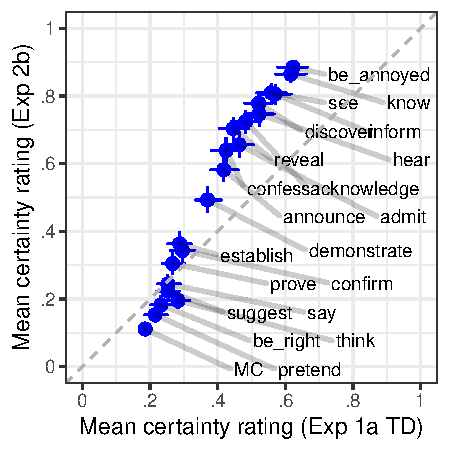
\includegraphics[width=\textwidth]{../../results/projection-comparisons/graphs/projection-comparison-35}
\caption{Exp.~2b vs.\ Exp.~1a TD.}
\label{f-projcomp1}
\end{subfigure}
\begin{subfigure}{.33\textwidth}
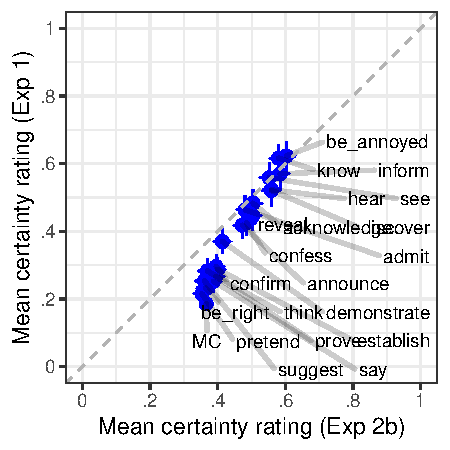
\includegraphics[width=\textwidth]{../../results/projection-comparisons/graphs/projection-comparison-39}
\caption{Exp.~1 vs.\ Exp.~2b.}
\label{f-projcomp2}
\end{subfigure}
\begin{subfigure}{.33\textwidth}
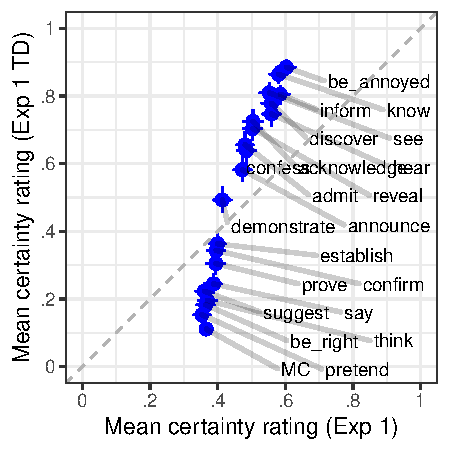
\includegraphics[width=\textwidth]{../../results/projection-comparisons/graphs/projection-comparison-59}
\caption{Exp.~1a TD vs.\  Exp.~1.}
\label{f-projcomp3}
\end{subfigure}
\caption{Comparisons of mean by-predicate certainty ratings from Exp.~1, Exp.~2b, and Tonhauser \& Degen's Exp.~1a (abbreviated `Exp.~1a TD'). Error bars indicate 95\% bootstrapped confidence intervals. Range of means from current experiments appears compressed compared to that of Tonhauser \& Degen because means are collapsed across fact type.}
\label{f-projection-comparisons}
\end{figure}

\newpage
\section{Experiment 2 supplements}\label{a-exp2}

The control items in Exp.~2a are given in (\ref{control2}).

\begin{exe}
\ex\label{control2}
\begin{xlist}
\ex {\bf Fact:} Barry lives in Germany. \\ How likely is it that Barry lives in Europe?
\ex {\bf Fact:} Tammy is a rabbit. \\ How likely is it that Tammy speaks Italian and Greek?
\end{xlist}
\end{exe}

\figref{f-prior-2a} shows the mean prior probabilities of the 20 contents by fact. Participants' ratings are given as light dots. The mean prior probability rating for each content was higher when the content was presented with the higher probability fact than when it was presented with the lower probability fact.

\begin{figure}[h!]
\centering
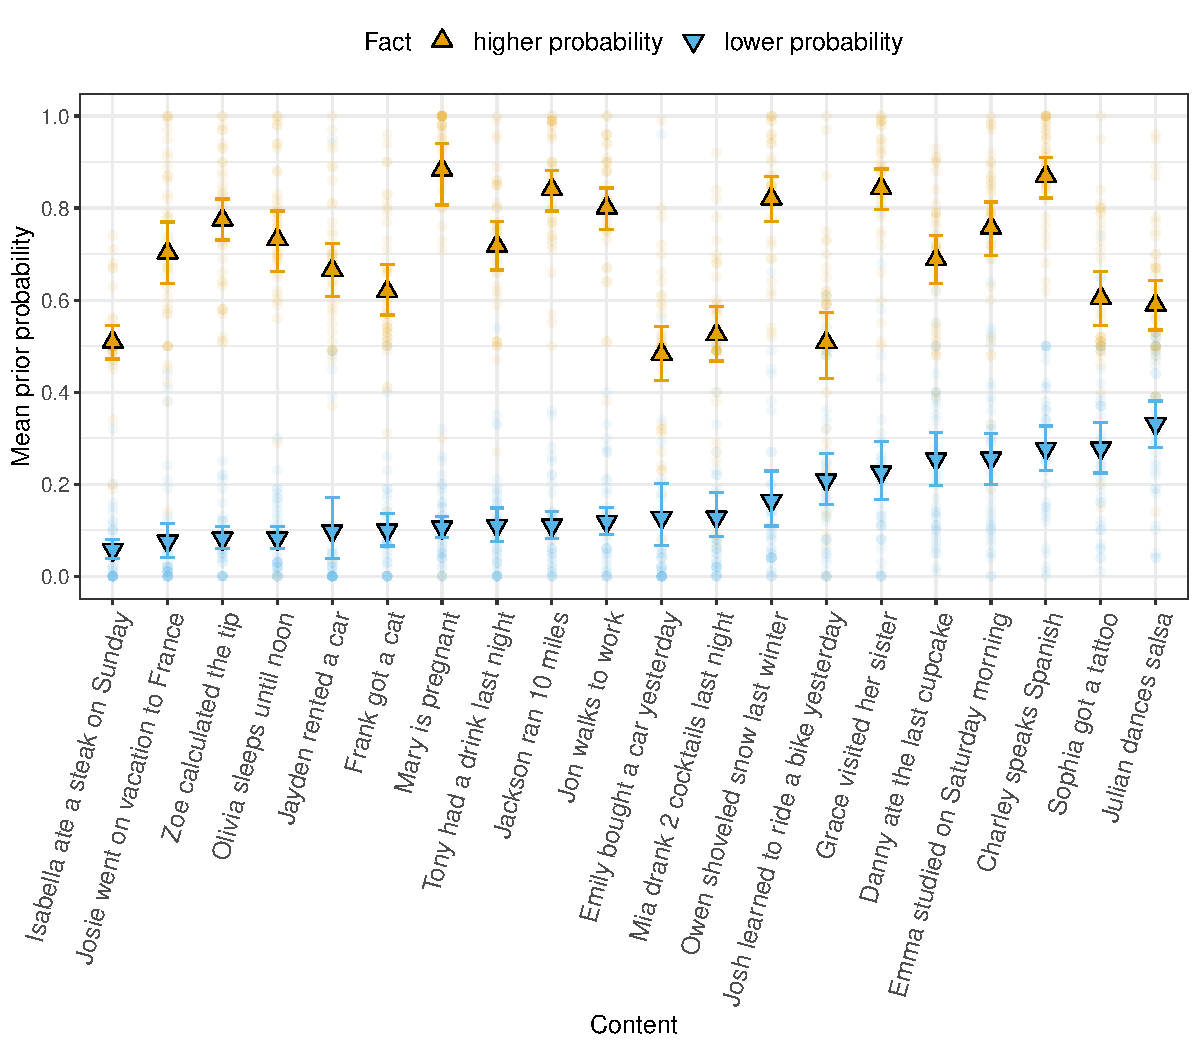
\includegraphics[width=.75\paperwidth]{../../results/1-prior/graphs/prior-ratings}
\caption{Mean prior probability by content and fact in Exp.~2a. Error bars indicate 95\% bootstrapped confidence intervals. Light dots indicate participants' ratings.} 
\label{f-prior-2a}
\end{figure}

\newpage
\section{Item variability in prior probability ratings}\label{app:prior-item}

\figref{fig:item-prior} shows by-item histograms of prior probability ratings.

\begin{figure}[h!]
\centering
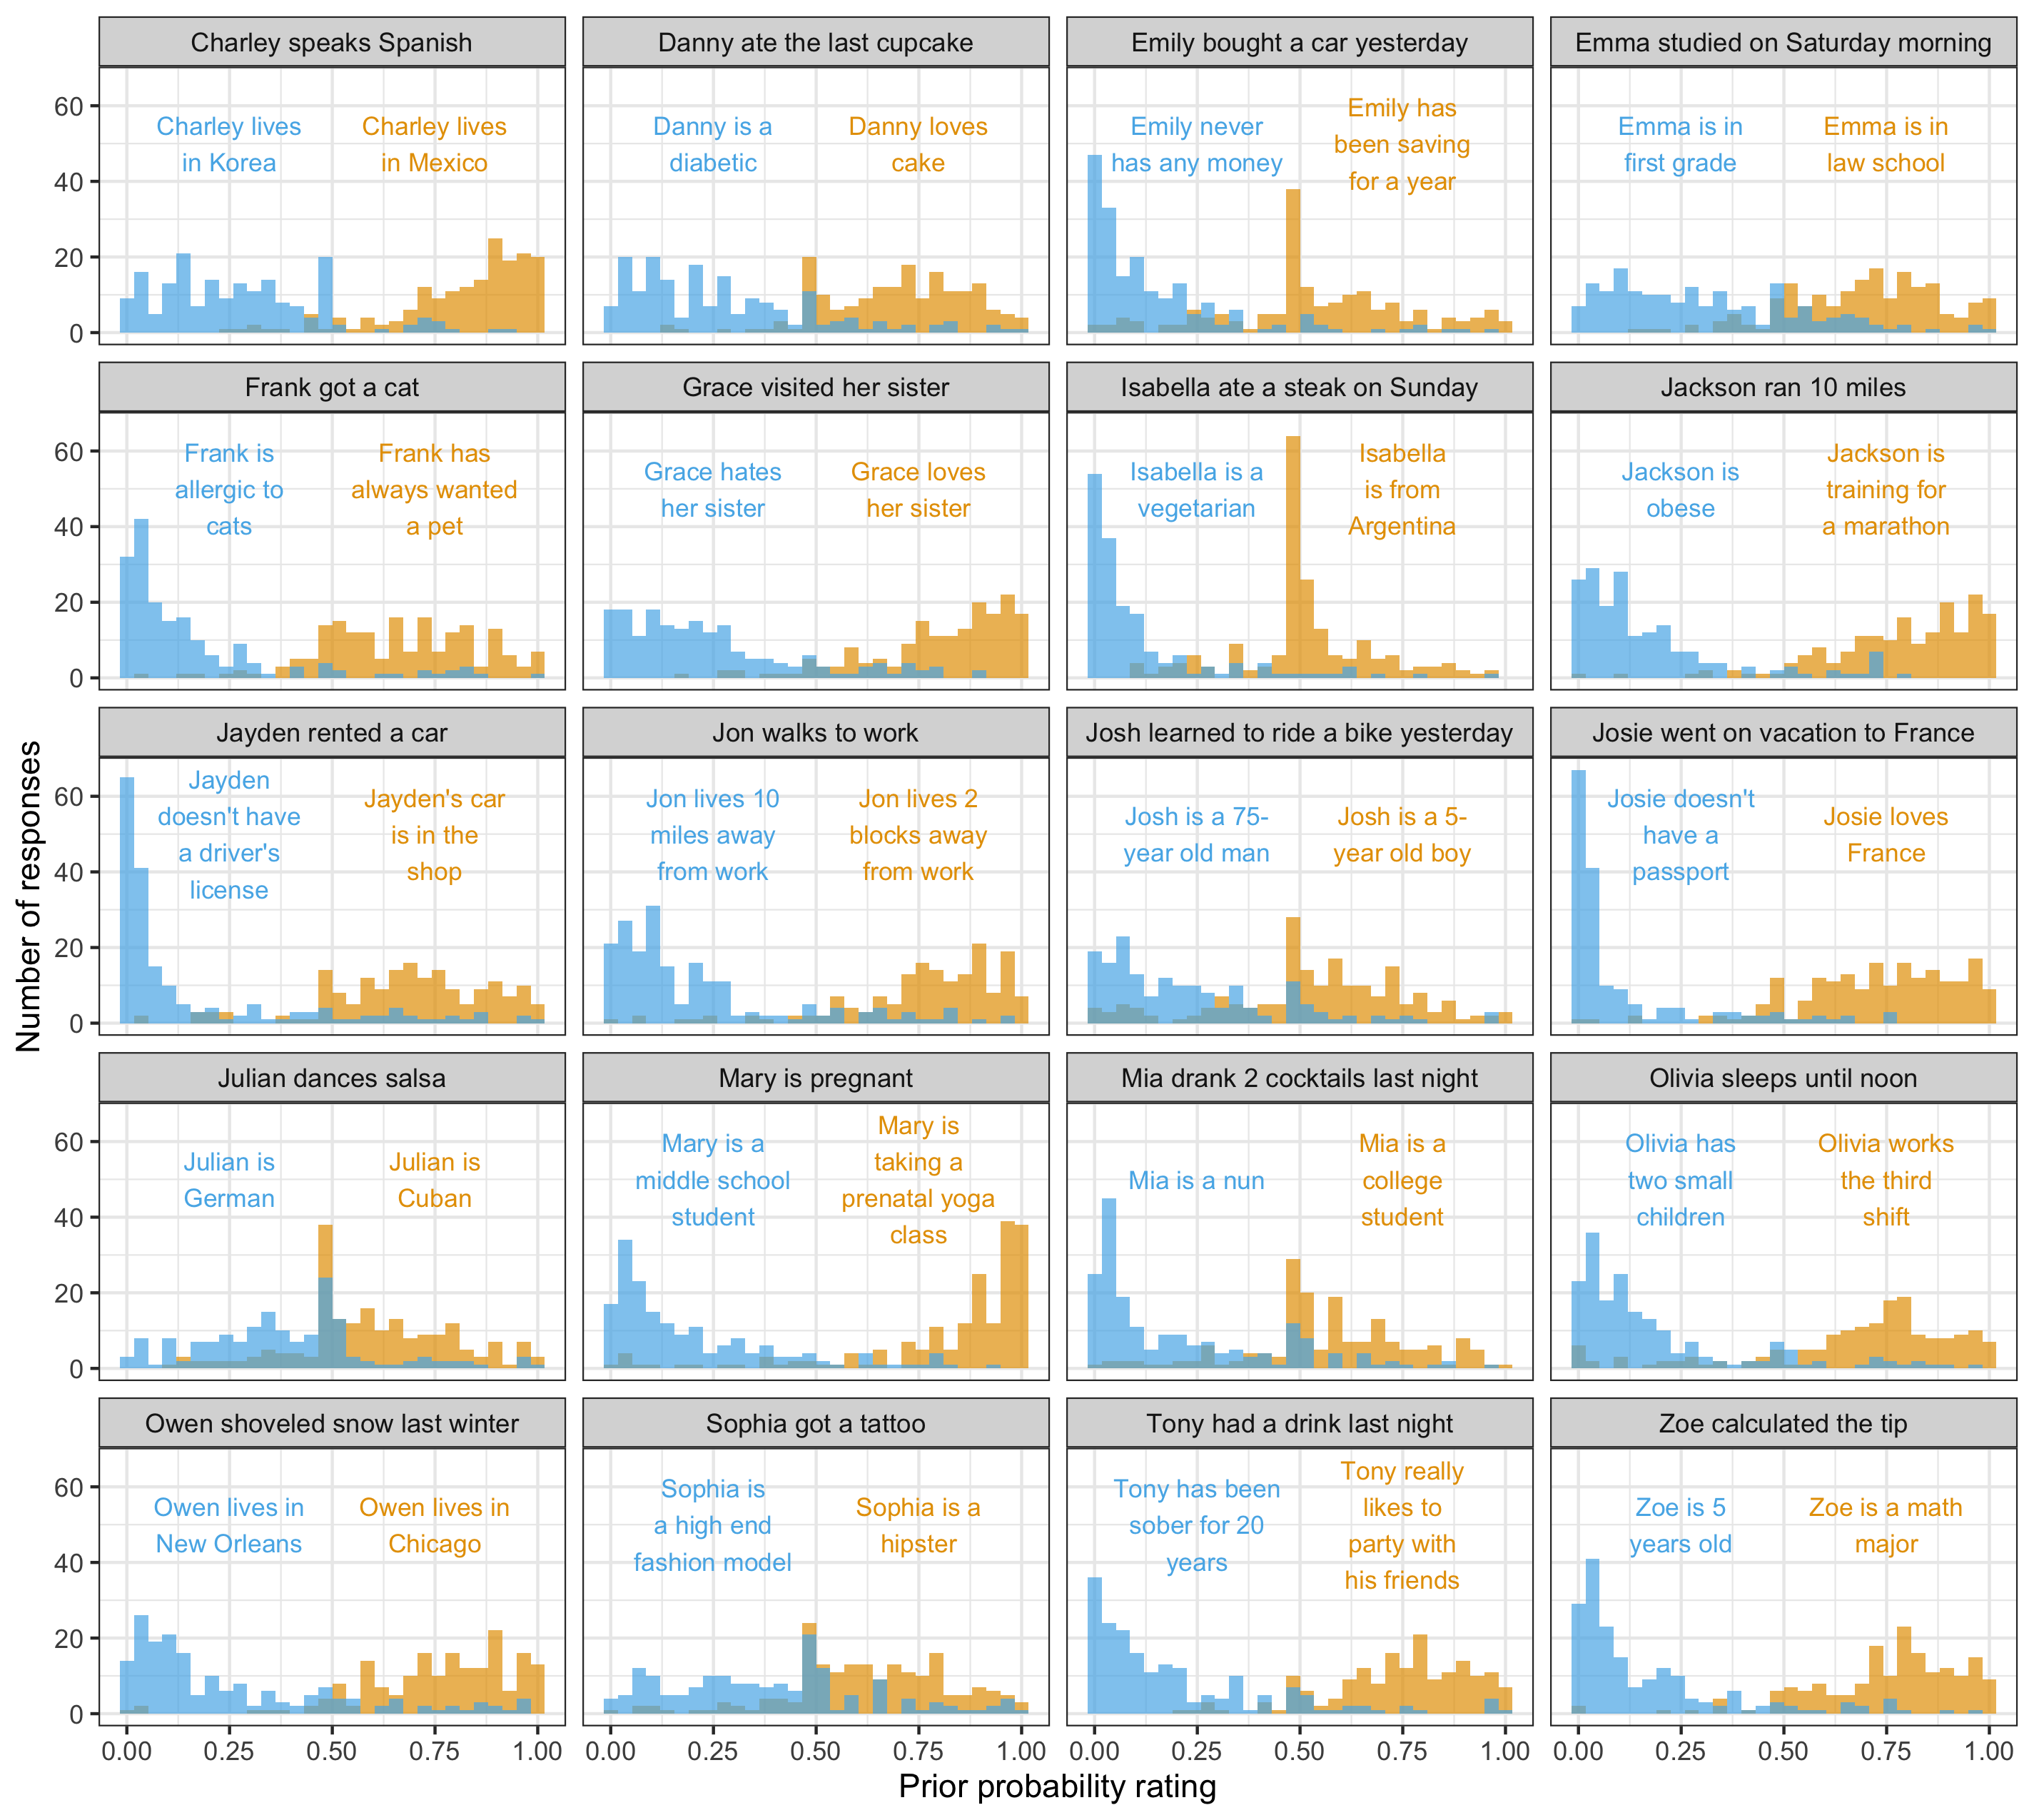
\includegraphics[width=\textwidth]{../../results/1-prior/graphs/item-variability-prior}
\caption{By-item histograms of prior probability ratings. Colors indicate whether the fact resulted in  lower (blue) vs.~higher (orange) prior probability ratings for the content indicated in the facet label.} 
\label{fig:item-prior}
\end{figure}

\bibliographystyle{apacite}
\bibliography{../../bibliography}

\end{document}

